% !TeX program = pdflatex
\documentclass[11pt,a4paper]{article}

% =========================================================
% PACKAGES (FAST)
% =========================================================
\usepackage[T1]{fontenc}
\usepackage[utf8]{inputenc}
\usepackage[english]{babel}

\usepackage{geometry}
\geometry{margin=2.2cm}

\usepackage{amsmath,amssymb,mathtools}
\usepackage{microtype}
\usepackage{lmodern}
\usepackage{parskip}

\usepackage{xcolor}
\usepackage{hyperref}
\usepackage{booktabs}
\usepackage{tabularx}
\usepackage{enumitem}

\usepackage{tcolorbox}
\tcbuselibrary{skins,breakable}

\usepackage{tikz}
\usetikzlibrary{arrows.meta}

% =========================================================
% COLORS
% =========================================================
\definecolor{Navy}{HTML}{061C3A}
\definecolor{Panel}{HTML}{0B2A4D}
\definecolor{Line}{HTML}{244A74}
\definecolor{Text}{HTML}{EAF2FF}
\definecolor{Muted}{HTML}{A9BBDC}

\definecolor{Delta}{RGB}{0,160,255}     % directional
\definecolor{Gamma}{RGB}{60,220,120}    % convexity
\definecolor{Theta}{RGB}{255,90,90}     % carry
\definecolor{Vega}{RGB}{190,120,255}    % implied vol

\hypersetup{
  colorlinks=true,
  linkcolor=Delta,
  urlcolor=Delta
}

% =========================================================
% BOXES (few, fast)
% =========================================================
\newtcolorbox{defbox}[1][]{
  enhanced, breakable,
  colback=white,
  colframe=Line,
  boxrule=0.8pt,
  arc=2mm,
  left=3mm,right=3mm,top=2mm,bottom=2mm,
  title=\textbf{Definition},
  #1
}
\newtcolorbox{insightbox}[1][]{
  enhanced, breakable,
  colback=white,
  colframe=black!12,
  boxrule=0.7pt,
  arc=2mm,
  left=3mm,right=3mm,top=2mm,bottom=2mm,
  title=\textbf{Practical insight},
  #1
}
\newtcolorbox{warningbox}[1][]{
  enhanced, breakable,
  colback=white,
  colframe=Theta,
  boxrule=0.9pt,
  arc=2mm,
  left=3mm,right=3mm,top=2mm,bottom=2mm,
  title=\textbf{Pitfall / risk},
  #1
}
\newtcolorbox{atlasbox}[1][]{
  enhanced, breakable,
  colback=Panel,
  colframe=Line,
  boxrule=0.8pt,
  arc=2mm,
  left=3mm,right=3mm,top=2.2mm,bottom=2.2mm,
  #1
}
\newtcolorbox{subcatbox}[2][]{
  enhanced, breakable,
  colback=white,
  colframe=#2,
  boxrule=0.9pt,
  arc=2mm,
  left=3mm,right=3mm,top=2mm,bottom=2mm,
  #1
}

% =========================================================
% TAGS (FAST: fcolorbox)
% =========================================================
\newcommand{\Tag}[2]{%
  \begingroup
  \setlength{\fboxsep}{2.2pt}%
  \fcolorbox{#2}{#2!10}{\textcolor{#2}{\scriptsize\bfseries #1}}%
  \endgroup
}
\newcommand{\GreekSig}[4]{%
  \Tag{$\Delta$\,#1}{Delta}\;
  \Tag{$\Gamma$\,#2}{Gamma}\;
  \Tag{$\Theta$\,#3}{Theta}\;
  \Tag{$\nu$\,#4}{Vega}%
}
\newcommand{\Primary}[1]{\Tag{Primary: #1}{#1}}

% =========================================================
% STRATEGY ENTRY (no tcolorbox per strategy -> fast)
% =========================================================
\newcommand{\Strat}[6]{%
\textbf{#1}\hfill \Primary{#2}\\
\textbf{Greek signature (typical at initiation):} #3\\
\textbf{Structure:} #4\\
\textbf{What you are trading:} #5\\
\textbf{Key risks / notes:} #6\\[1.2mm]
}

% =========================================================
% LIGHTWEIGHT PAYOFF DRAWING MACROS (NO PGFPLOTS)
% =========================================================
\newcommand{\PayoffAxes}[3]{% xmin xmax label
\draw[->,line width=0.7pt] (#1,0) -- (#2,0) node[below] {\small $S_T$};
\draw[->,line width=0.7pt] (0,-1.2) -- (0,2.2) node[left] {\small Payoff};
\node[anchor=west] at (#1,2.0) {\small\bfseries #3};
}
\newcommand{\StrikeMark}[1]{%
\draw[line width=0.6pt] (#1,-0.12) -- (#1,0.12);
\node[below] at (#1,-0.12) {\scriptsize $K$};
}

% =========================================================
% TITLE
% =========================================================
\title{\Huge\bfseries Options Strategies \& Greeks\\[1mm]
\Large A complete atlas (Novice $\rightarrow$ Expert) mapped to Delta, Gamma, Theta, Vega}
\author{}
\date{\today}

\begin{document}

% =========================================================
% COVER + DASHBOARD (dark, like your screenshot)
% =========================================================
\begin{titlepage}
\pagecolor{Navy}\color{Text}

\vspace*{1.5cm}
{\Huge\bfseries Options Strategy Atlas}\\[2mm]
{\Large\color{Muted}A “melting pot” of strategies mapped to the Greeks}\\[6mm]

\begin{atlasbox}
\textbf{Legend (dominant Greek driver)}\quad
\Tag{Delta / Direction}{Delta}\quad
\Tag{Gamma / Convexity}{Gamma}\quad
\Tag{Theta / Carry}{Theta}\quad
\Tag{Vega / Implied Vol}{Vega}

\vspace{1mm}
\color{Muted}\small
Dominant Greek means: the main risk factor you are deliberately taking (or hedging) \emph{most of the time}.
Greek signs are \emph{typical at initiation} (near ATM). They can change with spot, time, and volatility surface moves.
\end{atlasbox}

\vspace{4mm}

\begin{atlasbox}
\color{Text}
\begingroup
\renewcommand{\arraystretch}{1.15}
\begin{tabularx}{\textwidth}{@{}X X X X X@{}}
\toprule
\textbf{\Large Novice} & \textbf{\Large Intermediate} & \textbf{\Large Advanced} & \textbf{\Large Pro} & \textbf{\Large Expert}\\
\midrule
\textbf{\color{Muted}BASIC}\par
\textcolor{Delta}{Long Call}\par
\textcolor{Delta}{Long Put}\par
\vspace{1mm}
\textbf{\color{Muted}INCOME}\par
\textcolor{Theta}{Covered Call}\par
\textcolor{Theta}{Cash-Secured Put}\par
\vspace{1mm}
\textbf{\color{Muted}OTHER}\par
\textcolor{Vega}{Protective Put}\par

&
\textbf{\color{Muted}CREDIT SPREADS}\par
\textcolor{Theta}{Bull Put Spread}\par
\textcolor{Theta}{Bear Call Spread}\par
\vspace{1mm}
\textbf{\color{Muted}DEBIT SPREADS}\par
\textcolor{Delta}{Bull Call Spread}\par
\textcolor{Delta}{Bear Put Spread}\par
\vspace{1mm}
\textbf{\color{Muted}NEUTRAL}\par
\textcolor{Theta}{Iron Butterfly}\par
\textcolor{Theta}{Iron Condor}\par
\textcolor{Gamma}{Long Put Butterfly}\par
\textcolor{Gamma}{Long Call Butterfly}\par
\vspace{1mm}
\textbf{\color{Muted}CALENDAR SPREADS}\par
\textcolor{Vega}{Calendar Call Spread}\par
\textcolor{Vega}{Calendar Put Spread}\par
\textcolor{Vega}{Diagonal Call Spread}\par
\textcolor{Vega}{Diagonal Put Spread}\par

&
\textbf{\color{Muted}NAKED}\par
\textcolor{Theta}{Short Put}\par
\textcolor{Theta}{Short Call}\par
\vspace{1mm}
\textbf{\color{Muted}NEUTRAL}\par
\textcolor{Theta}{Short Straddle}\par
\textcolor{Theta}{Short Strangle}\par
\textcolor{Gamma}{Long Call Condor}\par
\textcolor{Gamma}{Long Put Condor}\par
\vspace{1mm}
\textbf{\color{Muted}DIRECTIONAL}\par
\textcolor{Vega}{Inverse Iron Butterfly}\par
\textcolor{Vega}{Inverse Iron Condor}\par
\textcolor{Theta}{Short Put Butterfly}\par
\textcolor{Theta}{Short Call Butterfly}\par
\textcolor{Gamma}{Straddle}\par
\textcolor{Gamma}{Strangle}\par
\vspace{1mm}
\textbf{\color{Muted}RATIO / BROKEN WING}\par
\textcolor{Gamma}{Call Ratio Backspread}\par
\textcolor{Gamma}{Put Ratio Backspread}\par
\textcolor{Gamma}{Call Broken Wing}\par
\textcolor{Gamma}{Put Broken Wing}\par
\textcolor{Theta}{Inverse Call Broken Wing}\par
\textcolor{Theta}{Inverse Put Broken Wing}\par
\vspace{1mm}
\textbf{\color{Muted}OTHER}\par
\textcolor{Delta}{Collar}\par

&
\textbf{\color{Muted}INCOME}\par
\textcolor{Theta}{Covered Short Straddle}\par
\textcolor{Theta}{Covered Short Strangle}\par
\vspace{1mm}
\textbf{\color{Muted}DIRECTIONAL}\par
\textcolor{Theta}{Short Call Condor}\par
\textcolor{Theta}{Short Put Condor}\par
\vspace{1mm}
\textbf{\color{Muted}LADDERS}\par
\textcolor{Delta}{Bull Call Ladder}\par
\textcolor{Delta}{Bear Call Ladder}\par
\textcolor{Delta}{Bull Put Ladder}\par
\textcolor{Delta}{Bear Put Ladder}\par
\vspace{1mm}
\textbf{\color{Muted}OTHER}\par
\textcolor{Theta}{Jade Lizard}\par
\textcolor{Theta}{Reverse Jade Lizard}\par

&
\textbf{\color{Muted}RATIO SPREADS}\par
\textcolor{Theta}{Call Ratio Spread}\par
\textcolor{Theta}{Put Ratio Spread}\par
\vspace{1mm}
\textbf{\color{Muted}SYNTHETIC}\par
\textcolor{Delta}{Long Synthetic Future}\par
\textcolor{Delta}{Short Synthetic Future}\par
\textcolor{Delta}{Synthetic Put}\par
\vspace{1mm}
\textbf{\color{Muted}ARBITRAGE}\par
\textcolor{Delta}{Long Combo}\par
\textcolor{Delta}{Short Combo}\par
\vspace{1mm}
\textbf{\color{Muted}OTHER}\par
\textcolor{Gamma}{Strip}\par
\textcolor{Gamma}{Strap}\par
\textcolor{Gamma}{Guts}\par
\textcolor{Theta}{Short Guts}\par
\textcolor{Vega}{Double Diagonal}\par
\\
\bottomrule
\end{tabularx}
\endgroup
\end{atlasbox}

\vfill
{\small\color{Muted}Compiled to stay within Overleaf free compile limits: no pgfplots, lightweight TikZ only.}
\end{titlepage}

\nopagecolor
\color{black}

\tableofcontents
\newpage

% =========================================================
\section{1. Greeks: the mathematical language behind every strategy}

\subsection{1.1 Price as a function of state variables}
We treat an option value as a function
\[
V = V(S,t,\sigma,\ldots),
\]
where $S$ is the underlying price, $t$ is time, and $\sigma$ is an implied-volatility input.

\begin{defbox}
\textbf{Core Greeks (continuous-time view).}
\[
\Delta = \frac{\partial V}{\partial S},\qquad
\Gamma = \frac{\partial^2 V}{\partial S^2},\qquad
\Theta = \frac{\partial V}{\partial t},\qquad
\nu = \frac{\partial V}{\partial \sigma}.
\]
\end{defbox}

\begin{insightbox}
\textbf{Interpretation.}
\begin{itemize}[leftmargin=*,itemsep=1mm]
\item \Tag{Delta}{Delta}: directional exposure (small spot moves).
\item \Tag{Gamma}{Gamma}: convexity (how Delta changes when spot moves).
\item \Tag{Theta}{Theta}: time decay / carry (you earn it when short premium, you pay it when long premium).
\item \Tag{Vega}{Vega}: sensitivity to implied vol (level + term structure + skew effects).
\end{itemize}
\end{insightbox}

\subsection{1.2 The “long option vs short option” rule (baseline)}
\begin{insightbox}
Near ATM, at initiation:
\begin{itemize}[leftmargin=*,itemsep=1mm]
\item \textbf{Long options:} typically \GreekSig{(sign depends)}{+}{-}{+}.
\item \textbf{Short options:} typically \GreekSig{(sign depends)}{-}{+}{-}.
\end{itemize}
Spreads and multi-leg structures \emph{reshape} this bundle (cap Gamma, reduce Vega, create Theta with defined risk, etc.).
\end{insightbox}

\begin{warningbox}
\textbf{Greeks move.}
A “Theta strategy” can become a “Gamma emergency” when spot approaches a short strike near expiry.
Always think \textbf{state-dependent risk}.
\end{warningbox}

% =========================================================
\section{2. Quick payoff intuition (light graphs)}

\subsection{2.1 Long call vs long put (expiry payoff)}
\begin{center}
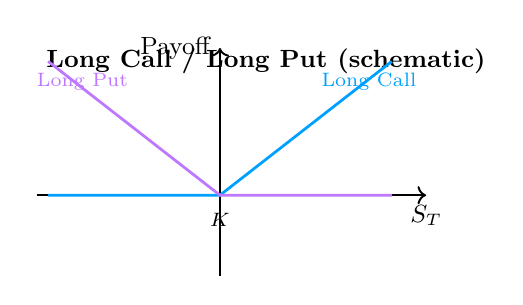
\begin{tikzpicture}[x=0.06\textwidth,y=0.85cm]
\PayoffAxes{-3.2}{3.6}{Long Call / Long Put (schematic)}
% K at x=0
\StrikeMark{0}
% long call
\draw[line width=1.0pt,Delta] (-3,0) -- (0,0) -- (3,2);
\node[Delta] at (2.6,1.7) {\scriptsize Long Call};
% long put
\draw[line width=1.0pt,Vega] (-3,2) -- (0,0) -- (3,0);
\node[Vega] at (-2.4,1.7) {\scriptsize Long Put};
\end{tikzpicture}
\end{center}

\subsection{2.2 Long straddle (expiry payoff)}
\begin{center}
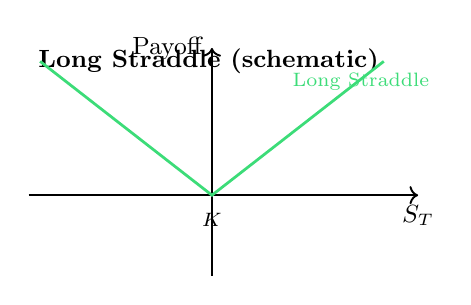
\begin{tikzpicture}[x=0.06\textwidth,y=0.85cm]
\PayoffAxes{-3.2}{3.6}{Long Straddle (schematic)}
\StrikeMark{0}
\draw[line width=1.0pt,Gamma] (-3,2) -- (0,0) -- (3,2);
\node[Gamma] at (2.6,1.7) {\scriptsize Long Straddle};
\end{tikzpicture}
\end{center}

\subsection{2.3 Iron condor (schematic payoff shape)}
\begin{center}
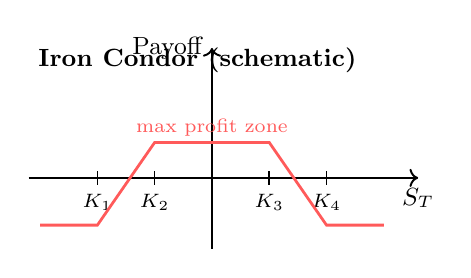
\begin{tikzpicture}[x=0.06\textwidth,y=0.75cm]
\PayoffAxes{-3.2}{3.6}{Iron Condor (schematic)}
% strikes: -2, -1, +1, +2
\draw[line width=0.6pt] (-2,-0.12)--(-2,0.12);
\draw[line width=0.6pt] (-1,-0.12)--(-1,0.12);
\draw[line width=0.6pt] (1,-0.12)--(1,0.12);
\draw[line width=0.6pt] (2,-0.12)--(2,0.12);
\node[below] at (-2,-0.12) {\scriptsize $K_1$};
\node[below] at (-1,-0.12) {\scriptsize $K_2$};
\node[below] at (1,-0.12) {\scriptsize $K_3$};
\node[below] at (2,-0.12) {\scriptsize $K_4$};

% payoff shape (credit condor)
\draw[line width=1.0pt,Theta]
(-3,-0.8) -- (-2,-0.8) -- (-1,0.6) -- (1,0.6) -- (2,-0.8) -- (3,-0.8);
\node[Theta] at (0,0.85) {\scriptsize max profit zone};
\end{tikzpicture}
\end{center}

% =========================================================
\section{3. Strategy catalogue (based on your reference screen)}
This section is the core: \textbf{every strategy} in the screen, and \textbf{which Greek(s)} it is designed to trade.

% =========================================================
\subsection{3.1 Novice}

\begin{subcatbox}[title=\textbf{Novice — BASIC}]{Delta}
\Strat{Long Call}{Delta}{\GreekSig{+}{+}{-}{+}}
{Buy 1 call.}
{Primarily directional upside (\Tag{Delta}{Delta}), plus convexity (\Tag{Gamma}{Gamma}) and long implied vol (\Tag{Vega}{Vega}).}
{You pay \Tag{Theta}{Theta}; far OTM calls can decay fast; Delta increases with spot due to Gamma.}

\Strat{Long Put}{Delta}{\GreekSig{-}{+}{-}{+}}
{Buy 1 put.}
{Directional downside hedge (\Tag{Delta}{Delta}) with crash convexity (\Tag{Gamma}{Gamma}) and long IV exposure (\Tag{Vega}{Vega}).}
{Insurance is expensive (Theta bleed). Best when downside move + IV expansion (equity skew).}
\end{subcatbox}

\begin{subcatbox}[title=\textbf{Novice — INCOME}]{Theta}
\Strat{Covered Call}{Theta}{\GreekSig{+}{-}{+}{-}}
{Long stock + short OTM call.}
{You sell time value (\Tag{Theta}{Theta}) on top of a long-Delta asset.}
{Upside is capped; short call adds short Vega and assignment risk; stock downside remains.}

\Strat{Cash-Secured Put}{Theta}{\GreekSig{+}{-}{+}{-}}
{Short put + cash reserved to buy at strike.}
{You collect carry (\Tag{Theta}{Theta}) and accept downside tail risk (short Gamma).}
{Large gap down dominates years of small gains; mark-to-market worsens when IV spikes.}
\end{subcatbox}

\begin{subcatbox}[title=\textbf{Novice — OTHER}]{Vega}
\Strat{Protective Put}{Vega}{\GreekSig{+}{+}{-}{+}}
{Long stock + long put.}
{You are buying downside convexity and IV (\Tag{Vega}{Vega}) as \emph{insurance}.}
{Costs Theta. Choose maturity/strike based on horizon (hedge vs speculation).}
\end{subcatbox}

% =========================================================
\subsection{3.2 Intermediate}

\begin{subcatbox}[title=\textbf{Intermediate — CREDIT SPREADS}]{Theta}
\Strat{Bull Put Spread}{Theta}{\GreekSig{+}{-}{+}{-}}
{Sell put $K_2$, buy put $K_1<K_2$ (net credit).}
{Theta harvesting with defined loss; still short Gamma/Vega but capped.}
{Fast losses on selloffs; avoid selling into events; size to survive worst-case move.}

\Strat{Bear Call Spread}{Theta}{\GreekSig{-}{-}{+}{-}}
{Sell call $K_1$, buy call $K_2>K_1$ (net credit).}
{Income from time decay; short gamma near the short call.}
{Rally risk; equity dividends can affect early assignment.}
\end{subcatbox}

\begin{subcatbox}[title=\textbf{Intermediate — DEBIT SPREADS}]{Delta}
\Strat{Bull Call Spread}{Delta}{\GreekSig{+}{+}{-}{+}}
{Buy call $K_1$, sell call $K_2>K_1$ (net debit).}
{Directional trade with reduced Vega/Theta vs naked call; capped upside.}
{You give up tail upside; performance depends on ending spot region.}

\Strat{Bear Put Spread}{Delta}{\GreekSig{-}{+}{-}{+}}
{Buy put $K_2$, sell put $K_1<K_2$ (net debit).}
{Directional downside with reduced Vega/Theta vs naked put; capped downside profit.}
{Selling the lower strike gives up deep-crash payoff.}
\end{subcatbox}

\begin{subcatbox}[title=\textbf{Intermediate — NEUTRAL}]{Theta}
\Strat{Iron Butterfly}{Theta}{\GreekSig{0}{-}{+}{-}}
{Short ATM straddle + long wings (defined risk).}
{Core thesis is positive Theta; you are short Gamma and short Vega around ATM.}
{Near expiry, tiny spot moves create large delta swings; needs active management.}

\Strat{Iron Condor}{Theta}{\GreekSig{0}{-}{+}{-}}
{Short OTM put spread + short OTM call spread.}
{Range-bound income: sell Theta, accept short Gamma/Vega (but defined wings).}
{Breakouts / event gaps are the enemy; manage early, not at the last day.}

\Strat{Long Put Butterfly}{Gamma}{\GreekSig{0}{+}{(often +)}{(often -)}}
{Put butterfly (buy 1, sell 2, buy 1) with symmetric strikes.}
{Targeted convexity around the body; often short vega; profit if spot pins near middle.}
{Very spot-location dependent; do not treat as “set and forget”.}

\Strat{Long Call Butterfly}{Gamma}{\GreekSig{0}{+}{(often +)}{(often -)}}
{Call butterfly (buy 1, sell 2, buy 1).}
{Same logic: gamma concentrated in a band; often short vega.}
{Pin risk and sensitivity explode close to expiry.}
\end{subcatbox}

\begin{subcatbox}[title=\textbf{Intermediate — CALENDAR SPREADS}]{Vega}
\Strat{Calendar Call Spread}{Vega}{\GreekSig{0}{(often -)}{(often +)}{+}}
{Sell short-dated call, buy longer-dated call (same strike).}
{A term-structure trade: typically long Vega, often positive Theta near ATM.}
{Front-month IV spikes (earnings) can hurt; delta changes if spot drifts away.}

\Strat{Calendar Put Spread}{Vega}{\GreekSig{0}{(often -)}{(often +)}{+}}
{Sell short-dated put, buy longer-dated put.}
{Same Vega thesis with put-side skew effects.}
{Selloffs stress the short put; assignment risk must be handled.}

\Strat{Diagonal Call Spread}{Vega}{\GreekSig{+}{(often -)}{(often +)}{+}}
{Calendar with different strikes (adds delta tilt).}
{Trade Vega/term structure plus a directional component.}
{More parameters: define which factor is your true thesis (spot vs IV).}

\Strat{Diagonal Put Spread}{Vega}{\GreekSig{-}{(often -)}{(often +)}{+}}
{Put diagonal (bearish tilt).}
{Vega + bearish tilt, sensitive to skew moves.}
{Strong downside move can dominate Greeks; stress scenarios.}
\end{subcatbox}

% =========================================================
\subsection{3.3 Advanced}

\begin{subcatbox}[title=\textbf{Advanced — NAKED}]{Theta}
\Strat{Short Put}{Theta}{\GreekSig{+}{-}{+}{-}}
{Sell 1 put (unhedged).}
{Pure Theta selling: short Vega and short Gamma on downside.}
{Tail risk is real. A single crash can wipe years of carry.}

\Strat{Short Call}{Theta}{\GreekSig{-}{-}{+}{-}}
{Sell 1 call (unhedged).}
{Theta selling with potentially unlimited upside loss.}
{Usually only done with strict limits or dynamic hedging.}
\end{subcatbox}

\begin{subcatbox}[title=\textbf{Advanced — NEUTRAL}]{Theta}
\Strat{Short Straddle}{Theta}{\GreekSig{0}{-}{+}{-}}
{Sell ATM call + sell ATM put.}
{Max theta / max short gamma near ATM: you sell volatility.}
{Gap risk + IV expansion are brutal; requires risk limits and hedging discipline.}

\Strat{Short Strangle}{Theta}{\GreekSig{0}{-}{+}{-}}
{Sell OTM call + sell OTM put.}
{Same theta thesis with wider range (less gamma than straddle).}
{Tail risk remains; mark-to-market worsens when IV rises.}

\Strat{Long Call Condor}{Gamma}{\GreekSig{0}{+}{(often 0)}{(often -)}}
{4-leg call condor (targeted payoff).}
{Gamma concentrated in a region; often short vega.}
{Path-dependent; Greeks flip as spot moves.}

\Strat{Long Put Condor}{Gamma}{\GreekSig{0}{+}{(often 0)}{(often -)}}
{Put condor.}
{Same: targeted convexity; often short vega.}
{Not intuitive: always plot and stress.}
\end{subcatbox}

\begin{subcatbox}[title=\textbf{Advanced — DIRECTIONAL (Long-vol variants)}]{Vega}
\Strat{Inverse Iron Butterfly}{Vega}{\GreekSig{0}{+}{-}{+}}
{Long straddle + short wings (reverse iron fly).}
{Long Gamma/Vega: you want movement and/or IV up.}
{Theta bleed; can be expensive; strong state dependence.}

\Strat{Inverse Iron Condor}{Vega}{\GreekSig{0}{+}{-}{+}}
{Buy OTM call spread + buy OTM put spread (debit).}
{Long Vega + long Gamma: breakout / realized vol trade.}
{If nothing happens, you lose (theta).}

\Strat{Straddle}{Gamma}{\GreekSig{0}{+}{-}{+}}
{Buy ATM call + buy ATM put.}
{Trade convexity + IV: big-move strategy.}
{Needs realized vol above implied (or IV expansion) to win.}

\Strat{Strangle}{Gamma}{\GreekSig{0}{+}{-}{+}}
{Buy OTM call + buy OTM put.}
{Cheaper convexity; needs larger move.}
{Lower gamma near spot, but still theta-negative.}

\Strat{Short Put Butterfly}{Theta}{\GreekSig{0}{-}{+}{(often 0)}}
{Sell a put butterfly (often for credit).}
{Theta harvesting with shaped risk; short gamma region near body.}
{Payoff can be non-obvious; worst region may sit between strikes.}

\Strat{Short Call Butterfly}{Theta}{\GreekSig{0}{-}{+}{(often 0)}}
{Sell a call butterfly (often for credit).}
{Similar: theta positive, short gamma around body.}
{Near expiry, risk becomes very “spiky”.}
\end{subcatbox}

\begin{subcatbox}[title=\textbf{Advanced — RATIO / BROKEN WING}]{Gamma}
\Strat{Call Ratio Backspread}{Gamma}{\GreekSig{+}{+}{-}{+}}
{Sell 1 call (near ATM) + buy 2 calls (OTM).}
{Upside convexity: long gamma beyond the long strike(s); often long vega.}
{There is typically a “valley” region around the short strike; manage carefully.}

\Strat{Put Ratio Backspread}{Gamma}{\GreekSig{-}{+}{-}{+}}
{Sell 1 put (near ATM) + buy 2 puts (lower).}
{Downside convexity + often long vega.}
{Slow drift can hurt; tail event helps.}

\Strat{Call Broken Wing}{Gamma}{\GreekSig{0}{+}{(often +)}{(often -)}}
{Asymmetric call butterfly: one wing moved further.}
{Targeted gamma in a region; sometimes designed for cheap entry/credit.}
{Asymmetry makes max-loss region less intuitive; always compute worst-case.}

\Strat{Put Broken Wing}{Gamma}{\GreekSig{0}{+}{(often +)}{(often -)}}
{Asymmetric put butterfly.}
{Same idea: shape payoff and reduce cost.}
{Still very spot-dependent; beware near expiry.}

\Strat{Inverse Call Broken Wing}{Theta}{\GreekSig{0}{-}{+}{(often 0)}}
{“Sell” the broken-wing structure (credit style).}
{Theta harvesting with non-linear risk.}
{Easy to misunderstand: plot it and identify max loss explicitly.}

\Strat{Inverse Put Broken Wing}{Theta}{\GreekSig{0}{-}{+}{(often 0)}}
{Inverse broken-wing on puts (credit style).}
{Theta strategy with shaped downside/upsides.}
{Sizing matters; can still be nasty in fast moves.}
\end{subcatbox}

\begin{subcatbox}[title=\textbf{Advanced — OTHER}]{Delta}
\Strat{Collar}{Delta}{\GreekSig{+}{(low)}{(varies)}{(varies)}}
{Long stock + long put + short call (financed hedge).}
{Primarily a Delta-risk shaping tool: keep exposure, cap upside, protect downside.}
{Short call introduces assignment and short vega; hedge effectiveness depends on strikes.}
\end{subcatbox}

% =========================================================
\subsection{3.4 Pro}

\begin{subcatbox}[title=\textbf{Pro — INCOME}]{Theta}
\Strat{Covered Short Straddle}{Theta}{\GreekSig{0}{-}{+}{-}}
{Short straddle + stock overlay (implementation varies).}
{Still mainly theta selling; stock overlay changes delta exposure.}
{Do not confuse “covered” with “safe”: gamma/vega risk remains.}

\Strat{Covered Short Strangle}{Theta}{\GreekSig{0}{-}{+}{-}}
{Short strangle + stock overlay.}
{Same thesis: carry harvesting with adjusted delta.}
{Tail risk remains; margin and hedging discipline required.}
\end{subcatbox}

\begin{subcatbox}[title=\textbf{Pro — DIRECTIONAL}]{Theta}
\Strat{Short Call Condor}{Theta}{\GreekSig{0}{-}{+}{-}}
{Call-side condor credit.}
{Theta income with defined wings; short gamma around short strikes.}
{Rally can push you into the short side quickly.}

\Strat{Short Put Condor}{Theta}{\GreekSig{0}{-}{+}{-}}
{Put-side condor credit.}
{Same structure, downside skew is the common risk factor.}
{Downside tail remains even if defined; size for worst-case.}
\end{subcatbox}

\begin{subcatbox}[title=\textbf{Pro — LADDERS}]{Delta}
\Strat{Bull Call Ladder}{Delta}{\GreekSig{+}{(often -)}{(often +)}{(often -)}}
{Typical idea: buy 1 call, sell 2 calls at higher strikes (variants exist).}
{Directional structure with short gamma beyond the highest short strike.}
{Naming is inconsistent across desks: always define legs explicitly.}

\Strat{Bear Call Ladder}{Delta}{\GreekSig{-}{(often -)}{(often +)}{(often -)}}
{Call ladder variant with bearish tilt (variants exist).}
{Often a directional + carry shape with short gamma region.}
{Plot required; risk can be unlimited depending on legs.}

\Strat{Bull Put Ladder}{Delta}{\GreekSig{+}{(often -)}{(often +)}{(often -)}}
{Put ladder with staged strikes (variants exist).}
{Directional bullish + carry with shaped downside exposure.}
{Can hide large tail risk; define max loss carefully.}

\Strat{Bear Put Ladder}{Delta}{\GreekSig{-}{(often -)}{(often +)}{(often -)}}
{Bearish ladder on puts (variants exist).}
{Directional bearish profile, can include short gamma zones.}
{Always compute payoff endpoints and worst-case.}
\end{subcatbox}

\begin{subcatbox}[title=\textbf{Pro — OTHER}]{Theta}
\Strat{Jade Lizard}{Theta}{\GreekSig{+}{-}{+}{-}}
{Short OTM put + short OTM call spread.}
{Income with “no upside risk” if credit covers call-spread width.}
{Downside risk is real (short put). Still short vega/gamma.}

\Strat{Reverse Jade Lizard}{Theta}{\GreekSig{-}{-}{+}{-}}
{Short OTM call + short OTM put spread.}
{Income with shaped downside (depending on credit condition).}
{Upside risk from short call; define the credit condition precisely.}
\end{subcatbox}

% =========================================================
\subsection{3.5 Expert}

\begin{subcatbox}[title=\textbf{Expert — RATIO SPREADS}]{Theta}
\Strat{Call Ratio Spread}{Theta}{\GreekSig{+}{(can flip)}{+}{-}}
{Typically 1x2 call ratio (buy 1, sell 2) or desk variant.}
{Often built for credit/theta but can create short gamma above a region.}
{Can have unlimited upside loss depending on strikes. Must be risk-limited.}

\Strat{Put Ratio Spread}{Theta}{\GreekSig{-}{(can flip)}{+}{-}}
{Typically 1x2 put ratio (buy 1, sell 2) or variant.}
{Carry profile with potential short gamma on large downside beyond region.}
{Downside tail can explode. Without hedging/limits this is dangerous.}
\end{subcatbox}

\begin{subcatbox}[title=\textbf{Expert — SYNTHETIC}]{Delta}
\Strat{Long Synthetic Future}{Delta}{\GreekSig{+}{0}{0}{0}}
{Buy call + sell put (same $K,T$).}
{Forward-like linear exposure: mainly Delta.}
{Carry/dividends/funding matter in practice.}

\Strat{Short Synthetic Future}{Delta}{\GreekSig{-}{0}{0}{0}}
{Sell call + buy put (same $K,T$).}
{Short forward-like exposure: mainly Delta.}
{Same practical risks: financing, borrow, assignment.}

\Strat{Synthetic Put}{Delta}{\GreekSig{-}{+}{-}{+}}
{Parity replication (e.g., long call + short stock + cash).}
{Economically similar to a long put (downside convexity).}
{Implementation depends on funding/borrow; check carry carefully.}
\end{subcatbox}

\begin{subcatbox}[title=\textbf{Expert — ARBITRAGE}]{Delta}
\Strat{Long Combo}{Delta}{\GreekSig{+}{0}{0}{0}}
{Commonly: long call + short put (often same $K,T$; variants exist).}
{Forward-like Delta; in variants (different strikes) it can be a skew trade.}
{Define your exact legs: same name, different risks depending on desk convention.}

\Strat{Short Combo}{Delta}{\GreekSig{-}{0}{0}{0}}
{Short call + long put (often same $K,T$).}
{Short forward-like Delta (or skew exposure in variants).}
{Funding and assignment practicalities dominate the real risk.}
\end{subcatbox}

\begin{subcatbox}[title=\textbf{Expert — OTHER}]{Gamma}
\Strat{Strip}{Gamma}{\GreekSig{-}{+}{-}{+}}
{Long 1 call + long 2 puts.}
{Long convexity with bearish bias (more downside sensitivity).}
{Theta-negative; used as downside crash convexity.}

\Strat{Strap}{Gamma}{\GreekSig{+}{+}{-}{+}}
{Long 2 calls + long 1 put.}
{Long convexity with bullish bias.}
{Still theta-negative; needs movement/IV.}

\Strat{Guts}{Gamma}{\GreekSig{0}{+}{-}{+}}
{Long ITM call + long ITM put.}
{Straddle-like but with more intrinsic; still long gamma/vega.}
{Expensive; not as “pure vol” as ATM straddle.}

\Strat{Short Guts}{Theta}{\GreekSig{0}{-}{+}{-}}
{Short ITM call + short ITM put.}
{Short vol carry with more intrinsic exposure.}
{Still big gap risk + big margin + short vega/gamma.}

\Strat{Double Diagonal}{Vega}{\GreekSig{0}{(often 0)}{+}{+}}
{Combine a call diagonal + put diagonal (common implementation).}
{Designed to be long Vega/term-structure while controlling Theta.}
{Highly surface-dependent (skew + term structure). Stress test scenarios.}
\end{subcatbox}

% =========================================================
\section{4. Final checklist: “which Greek am I really trading?”}
\begin{insightbox}
Before you place a trade, answer:
\begin{enumerate}[leftmargin=*,itemsep=1mm]
\item Is my dominant risk factor \Tag{Delta}{Delta}, \Tag{Gamma}{Gamma}, \Tag{Theta}{Theta}, or \Tag{Vega}{Vega}?
\item Where is my \textbf{short gamma region} (if any)? What happens if spot jumps there?
\item What happens if \textbf{implied vol shifts} and if \textbf{skew steepens}?
\item What happens if nothing happens (pure Theta carry)?
\item Do I know the \textbf{max loss} (defined-risk structures) or the margin worst-case (undefined)?
\end{enumerate}
\end{insightbox}

\end{document}
